\documentclass[10pt, a4paper]{article}
\usepackage{lrec}
\usepackage{multibib}
\newcites{languageresource}{Language Resources}
\usepackage{graphicx}
\usepackage{tabularx}
\usepackage{soul}
% for eps graphics

\usepackage{epstopdf}
\usepackage[latin1]{inputenc}

\usepackage{hyperref}
\usepackage{xstring}

\newcommand{\secref}[1]{\StrSubstitute{\getrefnumber{#1}}{.}{ }}

% Engado o da wikificación no apartado 11 (Copyrights)

% Hai que ver se vai levar algunha cita: se se quere citar con referencia ao que hai en http://sli.uvigo.gal/dbpedia/spotlight/ iso está feito con Lucene (é a primeira entrada que hai no xample.bib). Pero se se quere citar o modelo probabilístico novo é a segunda publicación do .bib

%% Igual habería que pensar na posibilidade de ofrecer o modelo no repositorio...

\title{Lingaliza: Processing Galician language with IXA--pipes \vspace*{.5\baselineskip} }

\name{Rodrigo Agerri $\textsuperscript{*}$, Xavier G\'omez Guinovart $\textsuperscript{**}$, German Rigau $\textsuperscript{*}$, Miguel Anxo Solla Portela $\textsuperscript{**}$}

\address{$\textsuperscript{*}$ IXA Reseach Group, University of the Basque Country  {\small $|$}
         $\textsuperscript{**}$ TALG Research Group, University of Vigo \\
         \{rodrigo.agerri, german.rigau\}@ehu.eus {\small $|$}
         \{xgg, miguelsolla\}@uvigo.es\\}


\abstract{
Each article must include an abstract of 150 to 200 words in Times New Roman
9 with interlinear spacing of 10 pt. The heading Abstract should be
centred, font Times New Roman 10 bold. This short abstract will also be used
for producing the Booklet of Abstracts (PDF) containing the abstracts of all
papers presented at the Conference. \\ \newline \Keywords{keyword1, keyword2,
keyword3} }

\begin{document}

\maketitleabstract

\section{Extended Abstract}

Each submitted abstract should be submitted on white A4 paper. The fully
justified text should be formatted in two parallel columns, each 8.25 cm wide,
and separated by a space of 0.63 cm. Left, right, and bottom margins should be
1.9 cm and the top margin 2.5 cm. The font for the main body of the text should
be Times New Roman 10 with interlinear spacing of 11 pt.

\subsection{General Instructions for the Submitted Abstract}

Each submitted abstract should be between \ul{a minimum of three and
a maximum of four pages including figures}.

\section{Corpus}

IXA-pipes statistical POS tagging and lemmatization (ixa-pipe-pos) for Galician is mainly based on CTG Galician Technical Corpus \citelanguageresource{ctg}\footnote{\url{http://sli.uvigo.gal/CTG/}}. The the IXA pipes POS-tagger language model is trained on a human-revised tagged subset of the CTG Corpus formed by 2,852,472 tokens, 105,986 sentences and 938 texts (news, scientific-technical divulgation, academic works, legal texts). 

The Galician dictionaries (galician.dict and gl-locutions.txt) contained in the distribution of the IXA pipes have been developed from several reference sources, including the Dicionario da Real Academia Galega\footnote{\url{http://academia.gal/dicionario/}}, the Vocabulario ortogr\'afico da lingua galega (VOLGa)\footnote{\url{http://www.realacademiagalega.org/recursos-volg}}, the Hunspell Spellchecker for Galician\footnote{\url{https://github.com/meixome/hunspell-gl}}, the Galician dictionary distributed by Apertium\footnote{\url{http://sourceforge.net/projects/apertium/}}, the Galician dictionary distributed by Freeling\footnote{\url{http://nlp.lsi.upc.edu/freeling/}}, and textual and lexical resources developed by the TALG research group. 
Both dictionaries (galician.dict and gl-locutions.txt) are distributed in a finite state automata format created using Morfologik\footnote{\url{https://github.com/morfologik/}} and are ready to use the IXA pipes POS-tagger to perform Galician dictionary-based lemmatization.

The collection of part-of speech tags used in the Galician corpus and dictionaries are based on the CTAG tagset developed by the TALG Group \cite{LM09}.

nerc

\section{DBpedia}

wikificacion

\section{Web applications}

Lingaliza

DContado

\section{Paper}

Each manuscript should be submitted on white A4 paper. The fully
justified text should be formatted in two parallel columns, each 8.25 cm wide,
and separated by a space of 0.63 cm. Left, right, and bottom margins should be
1.9 cm. and the top margin 2.5 cm. The font for the main body of the text should
be Times New Roman 10 with interlinear spacing of 12 pt.  Articles must be
between 4 and 8 pages in length, regardless of the mode of presentation (oral
or poster).

\subsection{General Instructions for the Final Paper}

Each paper is allocated between \ul{a minimum of four and a maximum of
eight pages including figures}. The unprotected PDF files will appear in the
on-line proceedings directly as received. Do not print the page number.

\section{Page Numbering}

\textbf{Please do not include page numbers in your article.} The definitive page
numbering of articles published in the proceedings will be decided by the
organising committee.

\section{Headings / Level 1 Headings}

Headings should be capitalised in the same way as the main title, and centred
within the column. The font used is Times New Roman 12 bold. There should
also be a space of 12 pt between the title and the preceding section, and
a space of 3 pt between the title and the text following it.

\subsection{Level 2 Headings}

The format for level 2 headings is the same as for level 1 Headings, with the
font Times New Roman 11, and the heading is justified to the left of the column.
There should also be a space of 6 pt between the title and the preceding
section, and a space of 3 pt between the title and the text following it.

\subsubsection{Level 3 Headings}

The format for level 3 headings is the same as for level 2 headings, except that
the font is Times New Roman 10, and there should be no space left between the
heading and the text. There should also be a space of 6 pt between the title and
the preceding section, and a space of 3 pt between the title and the text
following it.

%\subsubsection{Example of a sub-subsection with a long heading that will occupy two lines}
%
%Yet another example of a sub-subsection. Yet another example of a sub-subsection. Yet another example of a sub-subsection. Yet another example of a sub-subsection. Yet another example of a sub-subsection.

\section{Citing References in the Text}

\subsection{Bibliographical References}

All bibliographical references within the text should be put in between
parentheses with the author's surname followed by a comma before the date
of publication \cite{Martin-90}. If the sentence already includes the author's
name, then it is only necessary to put the date in parentheses:
\newcite{Martin-90}. When several authors are cited, those references should be
separated with a semicolon: \cite{Martin-90,CastorPollux-92}. When the reference
has more than three authors, only cite the name of the first author followed by
``et al.'' (e.g. \cite{Superman-Batman-Catwoman-Spiderman-00}).

\subsection{Language Resource References}

\subsubsection{When Citing Language Resources}

When citing language resources, we recommend to proceed in the same way to
bibliographical references, except that, in order to make them appear in
a separate section, you need to use the \texttt{\\citelanguageresource} tag.
Thus, a language resource should be cited as \citelanguageresource{speecon}.


\subsubsection{When Not Citing Any Language Resource}

When no language resource needs to be cited in the paper, you need to comment
out a few lines in the \texttt{.tex} file:

\begin{verbatim}
% \usepackage{multibib}
% \newcites{languageresource}{}
% \section{Language Resource References}
% \bibliographystylelanguageresource
%   {lrec}
% \bibliographylanguageresource{xample}
\end{verbatim}

\section{Figures \& Tables}
\subsection{Figures}

All figures should be centred and clearly distinguishable. They should never be
drawn by hand, and the lines must be very dark in order to ensure a high-quality
printed version. Figures should be numbered in the text, and have a caption in
Times New Roman 10 pt underneath. A space must be left between each figure and
its respective caption. 

Example of a figure enclosed in a box:

\begin{figure}[!h]
\begin{center}
%\fbox{\parbox{6cm}{
%This is a figure with a caption.}}
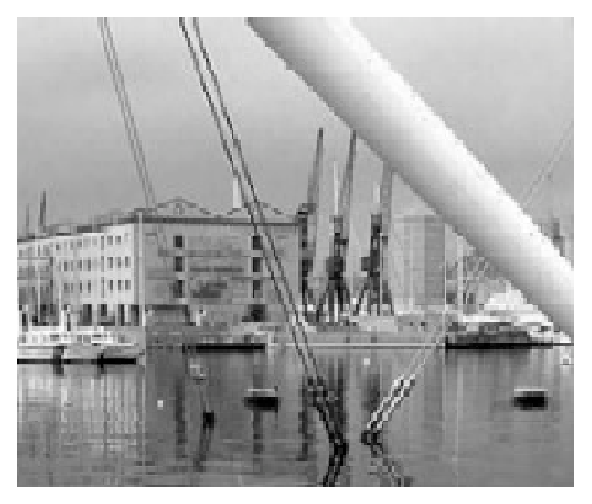
\includegraphics[scale=0.5]{image1.eps} 
\caption{The caption of the figure.}
\label{fig.1}
\end{center}
\end{figure}

Figure and caption should always appear together on the same page. Large figures
can be centred, using a full page.
%NB: an example of large figures is missing.  \newpage

\subsection{Tables}

The instructions for tables are the same as for figures.
%Two types of tables are distinguished: in-column and big tables that don't fit in the columns.
%\subsection{In-column tables}
%An example of an in-column table is presented here.
%
\begin{table}[!h]
\begin{center}
\begin{tabularx}{\columnwidth}{|l|X|}

      \hline
      Level&Tools\\
      \hline
      Morphology & Pitrat Analyser\\
      \hline
      Syntax & LFG Analyser (C-Structure)\\
      \hline
     Semantics & LFG F-Structures + Sowa's\\
     & Conceptual Graphs\\
      \hline

\end{tabularx}
\caption{The caption of the table}
 \end{center}
\end{table}

%\subsection{Big tables}
%
%An example of a big table which extends beyond the column and will
%float in the next page.
%
% \begin{table*}[ht]
% \begin{center}
% \begin{tabular}{|l|l|}
%
%       \hline
%       Level&Tools\\
%       \hline\hline
%       Morphology & Pitrat Analyser\\
%       Syntax & LFG Analyser (C-Structure)\\
%       Semantics & LFG F-Structures + Sowa's Conceptual Graphs  \\
%       \hline
%
% \end{tabular}
% \caption{The caption of the big table}
% \end{center}
% \end{table*}
%

\section{Footnotes}

Footnotes are indicated within the text by a number in
superscript\footnote{Footnotes should be in Times New Roman 9 pt, and appear at
the bottom of the same page as their corresponding number. Footnotes should also
be separated from the rest of the text by a horizontal line 5 cm long.}.

\section{Copyrights Lingaliza?}

The Lan\-gua\-ge Re\-sour\-ce and Evalua\-tion Con\-fe\-rence (LREC)
proceedings are published by the European Language Resources Association (ELRA).
They are available online from the conference website.


ELRA's policy is to acquire copyright for all LREC contributions. In assigning
your copyright, you are not forfeiting your right to use your contribution
elsewhere. This you may do without seeking permission and is subject only to
normal acknowledgement to the LREC proceedings. The LREC 2018 Proceedings are
licensed under CC-BY-NC, the Creative Commons Attribution-Non-Commercial 4.0
International License.

Since the Lucene version of DBpedia Spotlight\cite{isem2011mendesetal} was already working\footnote{Available at \url{http://sli.uvigo.gal/dbpedia/spotlight/}}, we also developed, adapting for the Galician language the model-quickstarter\footnote{\url{https://github.com/dbpedia-spotlight/model-quickstarter}} package, a new model for DBpedia Spotlight that allowed us to launch in Lingaliza the ixa-pipe-ned\footnote{\url{https://github.com/ixa-ehu/ixa-pipe-ned application}} and the ixa-pipe-wikify\footnote{\url{https://github.com/ixa-ehu/ixa-pipe-wikify}}. Both are part of IXA pipes and offer disambiguation based on DBpedia Spotlight, however, while ixa-pipe-wikify provides wikification by examining tokens, ixa-pipe-ned requires an input with Named Entity Recognition to perform the disambiguation directly on recognized entities.



\section{Conclusion}

Your submission of a finalised contribution for inclusion in the LREC
proceedings automatically assigns the above-mentioned copyright to ELRA.


\section{Acknowledgements}

Place all acknowledgements (including those concerning research grants and
funding) in a separate section at the end of the article.

\section{Providing References}

\subsection{Bibliographical References}
Bibliographical references should be listed in alphabetical order at the
end of the article. The title of the section, ``Bibliographical References'',
should be a level 1 heading. The first line of each bibliographical reference
should be justified to the left of the column, and the rest of the entry should
be indented by 0.35 cm.

The examples provided in Section \secref{main:ref} (some of which are fictitious
references) illustrate the basic format required for articles in conference
proceedings, books, journal articles, PhD theses, and chapters of books.

\subsection{Language Resource References}

Language resource references should be listed in alphabetical order at the end
of the article, in the \textbf{Language Resource References} section, placed after
the \textbf{Bibliographical References} section. The title of the ``Language Resource
References'' section, should be a level 1 heading. The first line of each
language resource reference should be justified to the left of the column, and
the rest of the entry should be indented by 0.35 cm. The example in Section 
\secref{lr:ref} illustrates the basic format required for language resources.

In order to be able to cite a language resource, it must be added to
the \texttt{.bib} file first, as a \texttt{@LanguageResource} item type, which
contains the following fields:

\begin{itemize}
    \item{\texttt{author}: the builder of the resource}
    \item{\texttt{title}: the name of the resource}
    \item{\texttt{publisher}: the publisher of the resource (project,
          organisation etc)}
    \item{\texttt{year}: year of the resource release}
    \item{\texttt{series}: more general resource set this language resource
          belongs to}
    \item{\texttt{edition}: version of the resource}
    \item{\texttt{islrn}: the International Standard Language Resource Number
          (ISLRN) of the resource\footnote{The ISLRN number is available from
          \texttt{http://islrn.org}}} 
\end{itemize}

If you want the full resource author name to appear in the citation, the
language resource author name should be protected by enclosing it between
\texttt{\{...\}}, as shown in the model \texttt{.bib} file.

\vspace{.3\baselineskip}

\section*{Appendix: How to Produce the \texttt{.pdf} Version}

In order to generate a PDF file out of the LaTeX file herein, when citing
language resources, the following steps need to be performed:

\begin{itemize}
    \item{Compile the \texttt{.tex} file once}
    \item{Invoke \texttt{bibtex} on the eponymous \texttt{.aux} file}
    \item{Invoke \texttt{bibtex} on the \texttt{languageresources.aux} file}
    \item{Compile the \texttt{.tex} file twice}
\end{itemize}

% \nocite{*}
\section{Bibliographical References}
\label{main:ref}

\bibliographystyle{lrec}
\bibliography{xample}


\section{Language Resource References}
\label{lr:ref}
\bibliographystylelanguageresource{lrec}
\bibliographylanguageresource{xample}

\end{document}
